\begin{frame}
    \frametitle{Transactions}
    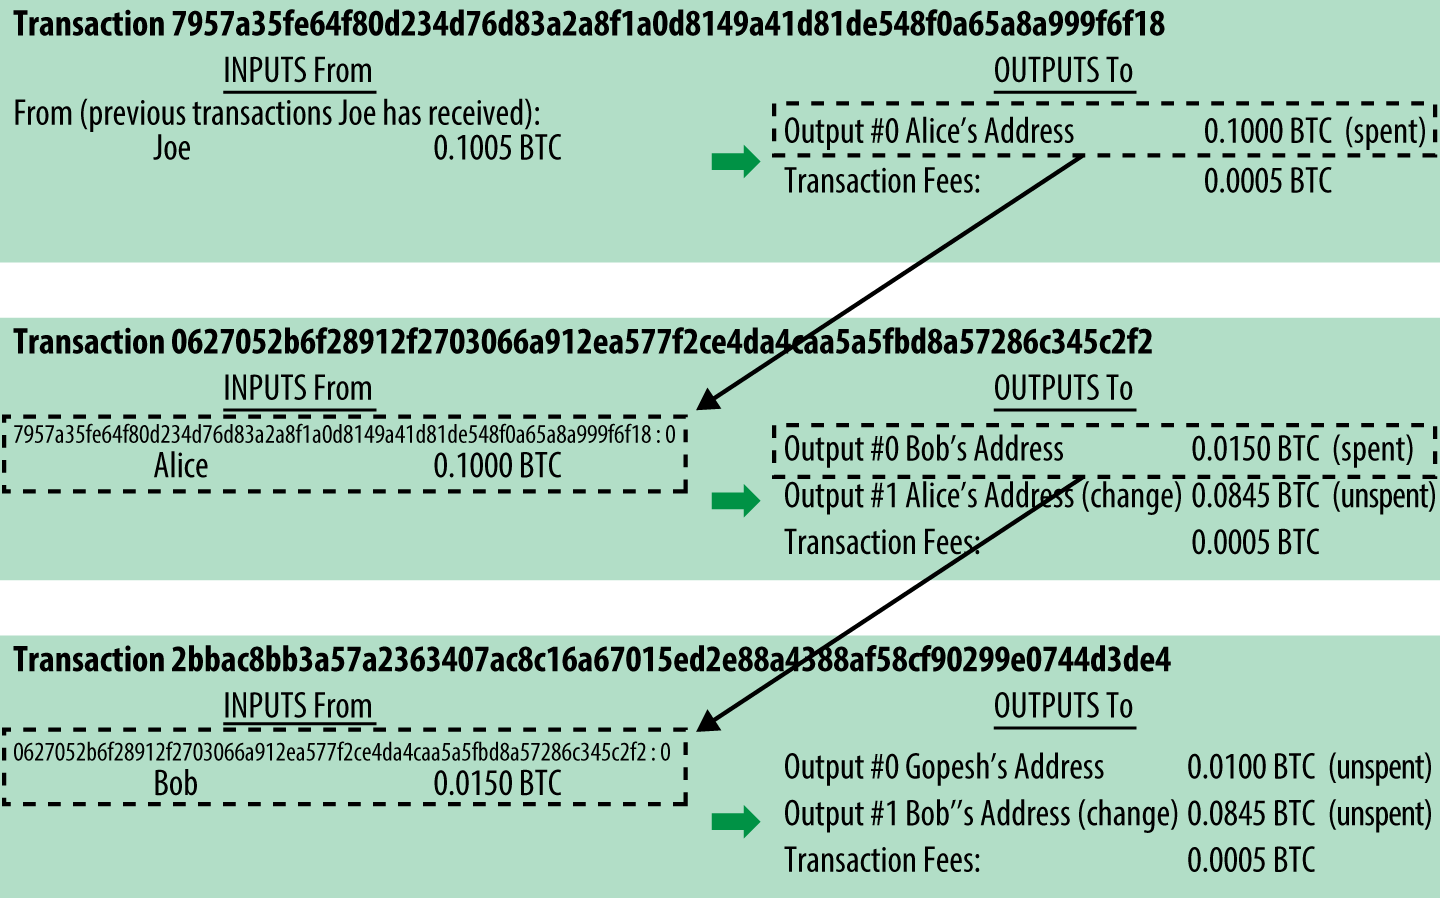
\includegraphics[scale=0.6]{./figures/mbc2_0204.png}
    \begin{itemize}
        \item \textbf{transaction input}: Where the coin is coming from, usually a previous transaction's output.
        \item \textbf{transaction output}: Assigns a new owner to the value by associating it with a key.
        \item \textbf{transaction fees}: Small payment collected by the miner.
    \end{itemize}
\end{frame}

\begin{frame}
    \frametitle{UTXO(Unspent Transaction Output)}
    \begin{itemize}
        \item UXTO is the fundamental building block of a bitcoin transaction.
        \item There are \alert{NO Accounts} in bitcoin, there are \alert{ONLY UTXO}.
    \end{itemize}
    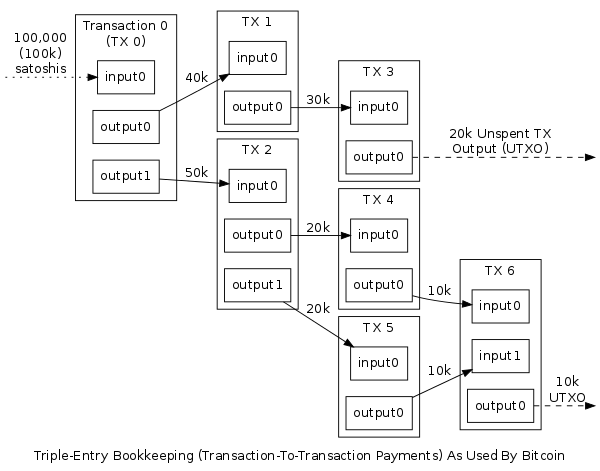
\includegraphics[scale=0.4]{./figures/en-transaction-propagation.png}
\end{frame}

\begin{frame}
    \frametitle{Transactions}
    \begin{columns}
        \begin{column}{0.5\textwidth}
            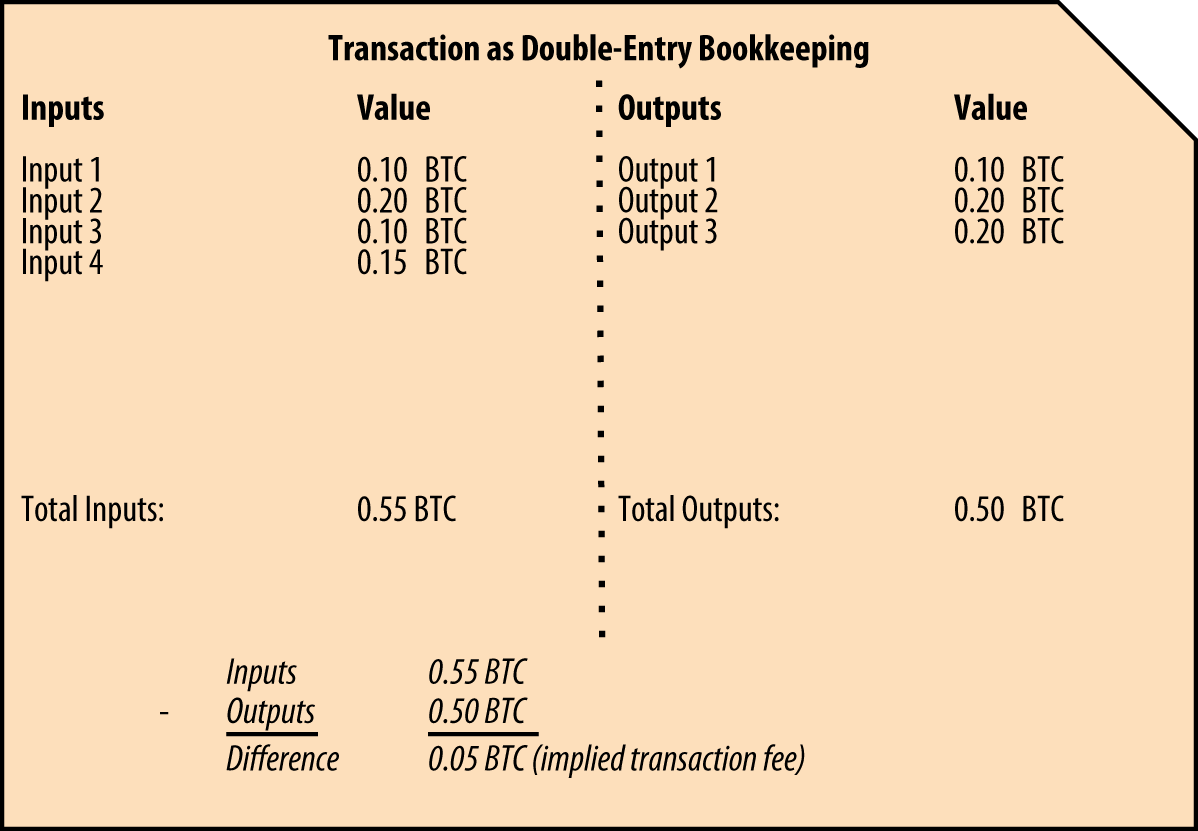
\includegraphics[scale=0.5]{./figures/mbc2_0203.png}
        \end{column}
        \begin{column}{0.5\textwidth}
            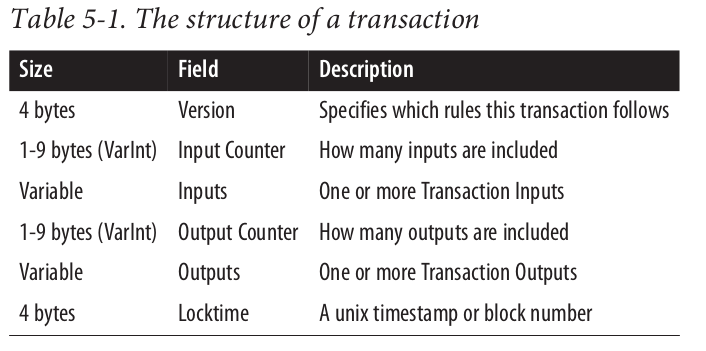
\includegraphics[scale=0.2]{./figures/transaction-data-structure.png}
        \end{column}
    \end{columns}
    \begin{itemize}
        \item A transaction is a transfer of bitcoin value that is broadcast to the network and collected into blocks.
        \item A transaction typically references previous transaction outputs as new transaction inputs and dedicates all input Bitcoin values to new outputs.
        \item Once transactions are buried under enough \alert{confirmations} they can be considered \alert{irreversible}.
    \end{itemize}
\end{frame}

\begin{frame}
    \frametitle{Regular Bitcoin Transaction}
    Transaction Data Structure:
    \begin{center}
        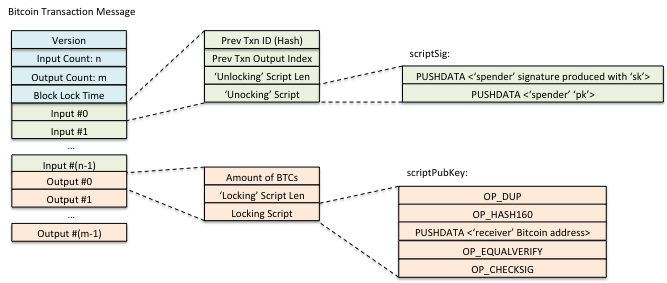
\includegraphics[scale=0.6]{./figures/bitcoin-transaction0.png} \\
    \end{center}
    \href{https://blockchain.info/tx/cca7507897abc89628f450e8b1e0c6fca4ec3f7b34cccf55f3f531c659ff4d79}{Transaction Example: The Famous Pizza Transaction}
\end{frame}

\begin{frame}
    \frametitle{Transaction Script: Lock + Unlock}
    \begin{itemize}
        \item Transaction Verification relies on \alert{Locking Script} and \alert{Unlocking Script}
        \item A Locking Script(\alert{scriptPubkey}) specifies the conditions that must be met to spend the output in the future.
        \item An Unlocking Script(\alert{scriptSig}) solves the conditions placed on an output by a Locking Script and allows the output to be spent.
        \item Every bitcoin client will validate transactions by executing the locking and unlocking scripts together.
    \end{itemize}
    \begin{center}
        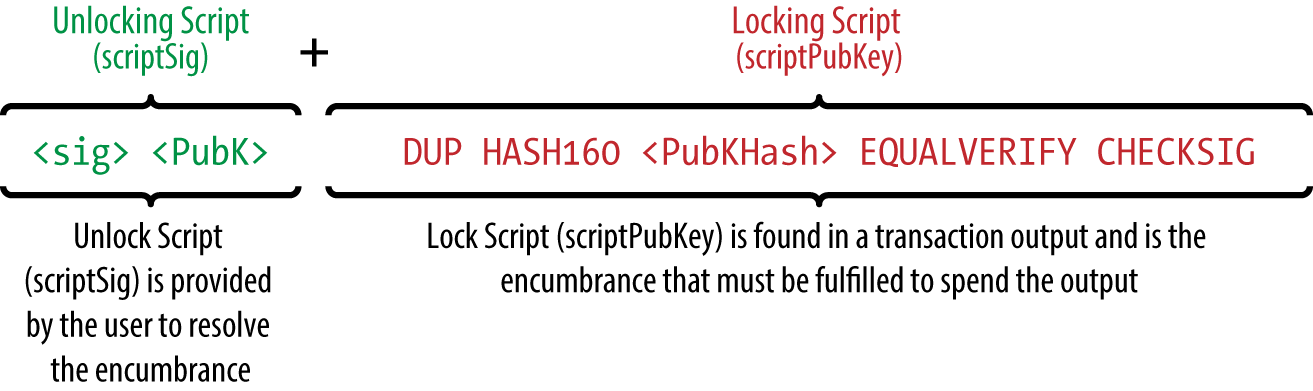
\includegraphics[scale=0.7]{./figures/mbc2_0603.png}
    \end{center}
\end{frame}

\begin{frame}
    \frametitle{Transaction Script}
    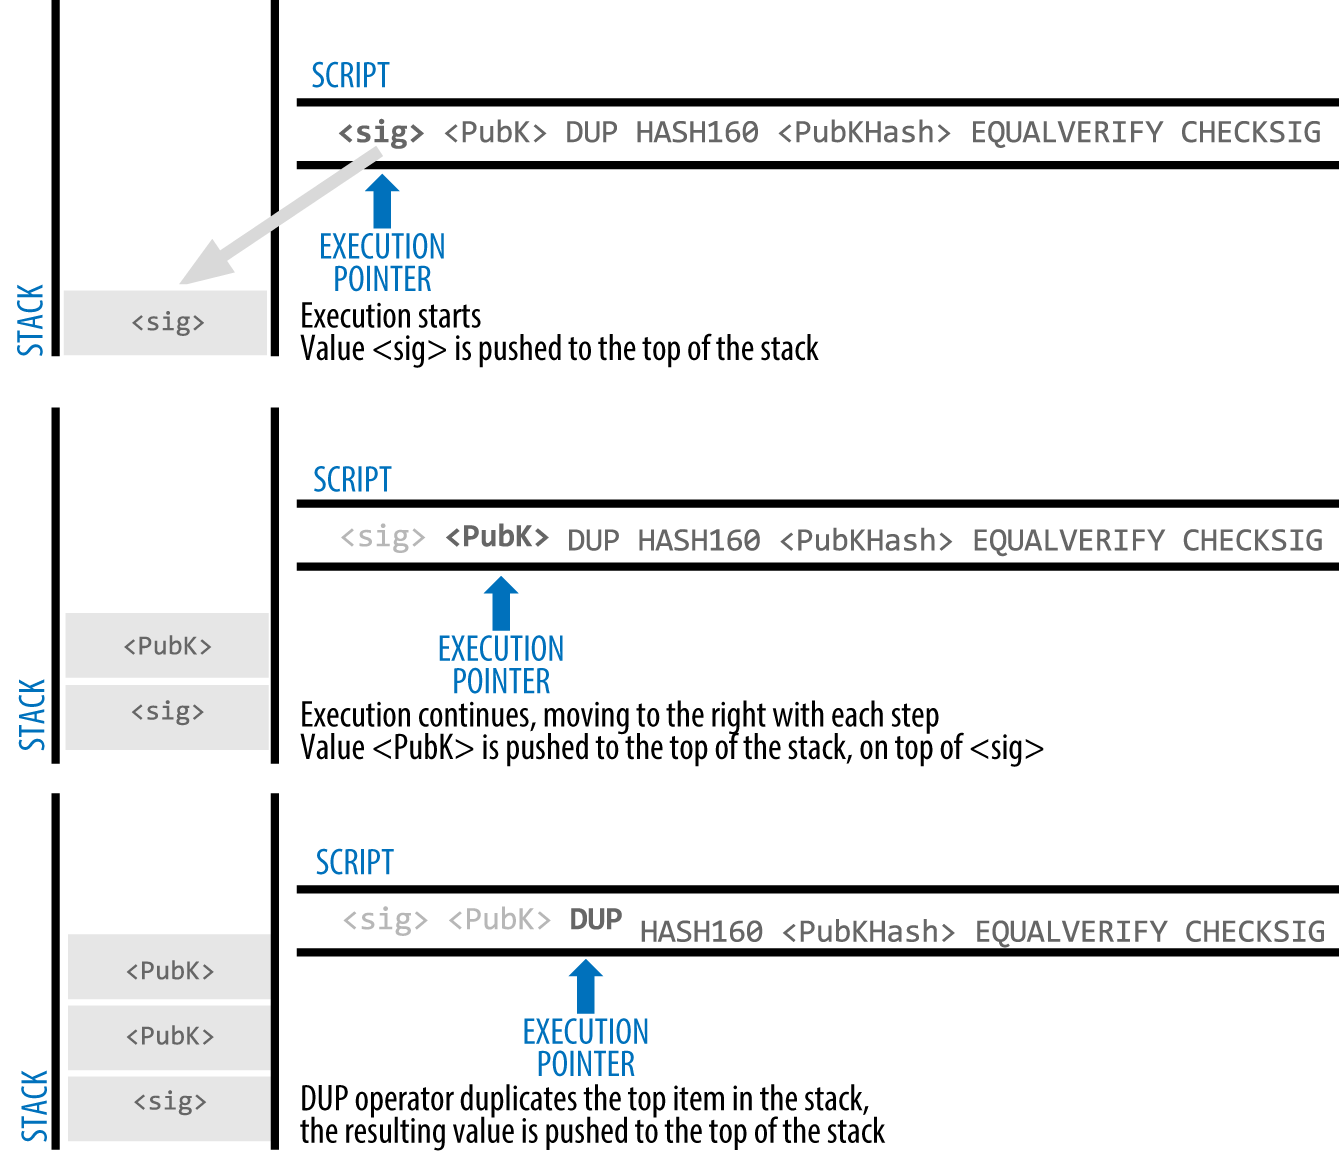
\includegraphics[scale=0.55]{./figures/mbc2_0605.png}
\end{frame}

\begin{frame}
    \frametitle{Transaction Script}
    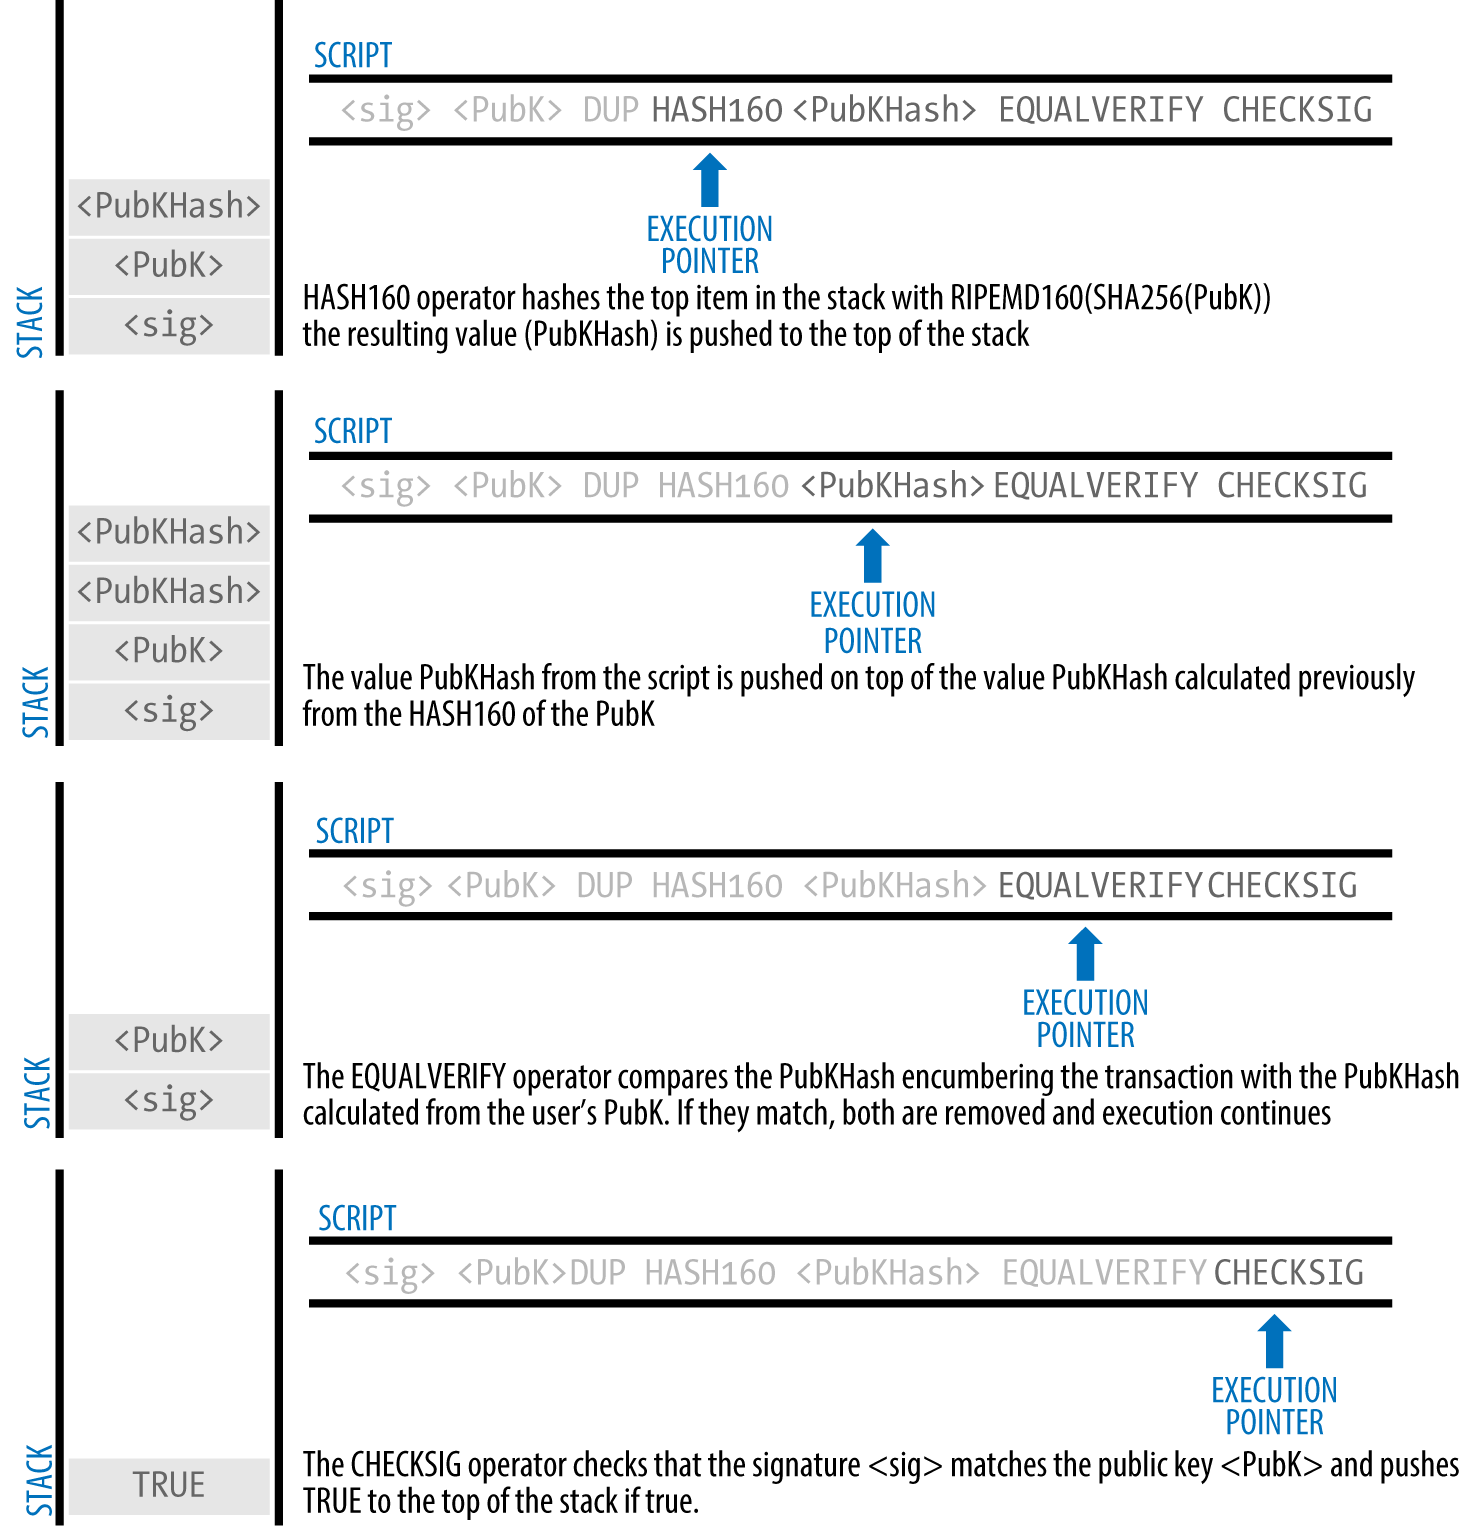
\includegraphics[scale=0.55]{./figures/mbc2_0606.png}
\end{frame}

\begin{frame}
    \frametitle{Bitcoin Transaction Verification}
    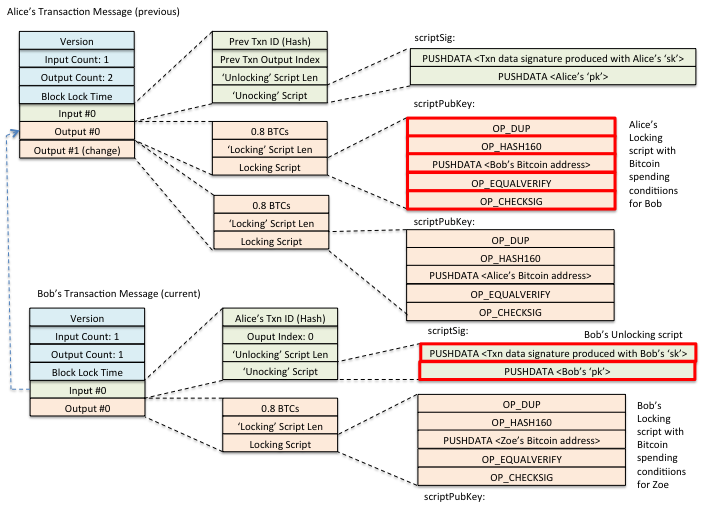
\includegraphics[scale=0.5]{./figures/bitcoin-transaction1.png}
\end{frame}
